\section{Operations Management of Scheduling and WIP}
\label{app:schedule}

\begin{table}[H]
\centering
\caption{Example menu. Job splitting shown in Table~\ref{tab:split}.}
\label{tab:menu}
\begin{tabular}{@{}lll@{}}
\toprule
Type      & Item                              & Characteristic \\ \midrule
Main meal & BLT sandwich & Made on day    \\
Snack     & Mixed nuts                        & Pre-packaged   \\
Treat     & Muffin                            & Made on day    \\
Drink     & Fruit juice                       & Pre-packaged   \\ \bottomrule
\end{tabular}
\end{table}

\begin{table}[H]
\centering
\caption{Task defining and staff scheduling for menu shown in Table~\ref{tab:menu}. Gantt chart illustrated in Figure~\ref{fig:gantt}}
\label{tab:split}
\begin{tabular}{C{1cm}L{3.8cm}C{1cm}C{1.2cm}C{1.2cm}C{2cm}C{2cm}}
\toprule
Task ID & Description & Staff & Serves & Cycle time (min) & Minimum total time & \multicolumn{1}{c}{Assigned staff}\\ \midrule
\multicolumn{7}{c}{BLT sandwich} \\
\multicolumn{7}{c}{(Qty = 120)} \\ \midrule
A1 & Prepare rolls & 3 & 1 & 1 & 40 & A, B, C \\
A2 & Cook and cut bacon & 2 & 5 & 5 & 60 & B, C \\
A3 & Wash lettuce & 1 & 6 & 2 & 40 & B \\
A4 & Slice tomatoes & 1 & 3 & 1 & 40 & C \\
A5 & Assemble \& package & 4 & 1 & 1 & 30 & A, B, C, D \\ \midrule
\multicolumn{7}{c}{Muffin} \\
\multicolumn{7}{c}{(Qty = 120)} \\ \midrule
B0 & Preheat oven & 1 & - & 20 & - & D \\
B1 & Prepare mix (5 min) & 1 & 24 & 5 & 25 & D \\
B2 & Bake (15 min) & 1 & 24 & 15 & 75 & D \\
B3 & Package & 1 & 1 & 0.25 & 30 & D \\ \midrule
\multicolumn{7}{c}{Assembly and Loading} \\
\multicolumn{7}{c}{(Qty = 120)} \\ \midrule
C1 & Labelling & 1 & 1 & 0.25 & 30 & E \\
C2 & Package pre-made & 1 & 1 & 0.5 & 60 & E \\
C3 & Finish packaging & 1 & 1 & 0.5 & 60 & E \\
C4 & Loading & 4 & 2 & 1 & 15 & A, B, C, D \\ \bottomrule
\end{tabular}
\end{table}

\begin{figure}[H]
    \centering
    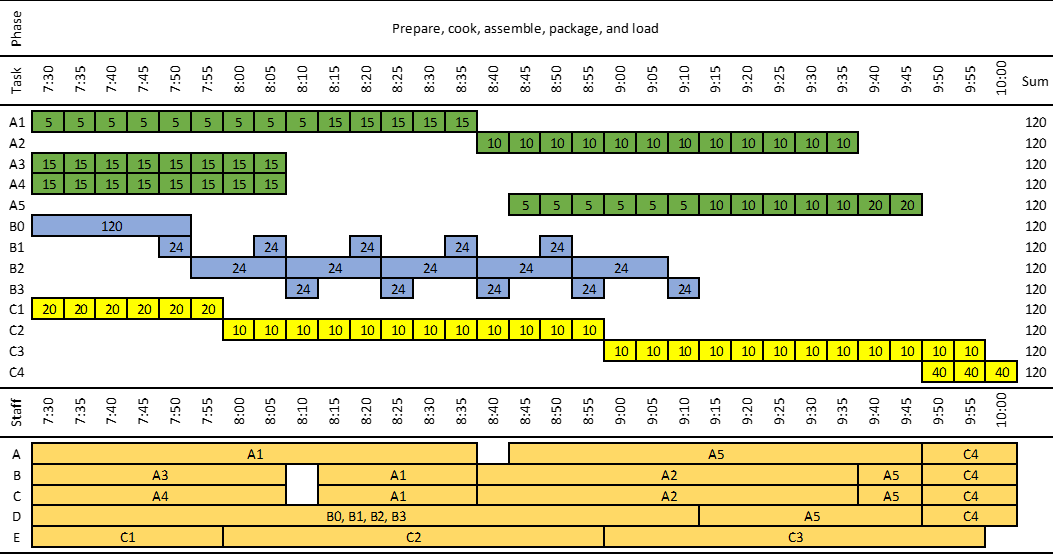
\includegraphics[angle=90, height=23cm]{ops_gantt.png}
    \caption{Operation scheduling example. Job descriptions and staff scheduling shown in Table~\ref{tab:split}.}
    \label{fig:gantt}
\end{figure}

